\documentclass{article}

\usepackage{amssymb}
\usepackage[english]{babel}
\usepackage{amsmath}
\usepackage[margin=1in]{geometry}
\usepackage{algorithm}
\usepackage{algpseudocode}
\usepackage{amsthm}
\usepackage{amsfonts}
\usepackage{graphicx, overpic}
\usepackage{color}
\usepackage{enumerate}
\usepackage{multicol}
\usepackage{mathrsfs}
\usepackage{mathabx}
\usepackage[T1]{fontenc}
\usepackage{pgfplots}
\usepackage{tikz}

\pgfplotsset{compat=1.17}

% Theorem Environments
\theoremstyle{plain}
\newtheorem{thm}{Theorem}[section]
\newtheorem{lemma}[thm]{Lemma}
\newtheorem{sublemma}[thm]{Sub-Lemma}
\newtheorem{prop}[thm]{Proposition}
\newtheorem{corollary}[thm]{Corollary}

% Definition Environments
\theoremstyle{definition}
\newtheorem*{definition}{Definition}
\newtheorem*{example}{Example}
\newtheorem*{remark}{Remark}
\newtheorem*{examples}{Examples}
\newtheorem*{obs}{Observation}
\newtheorem*{claim}{Claim}
\newtheorem*{assumption}{Assumption}
\newtheorem*{notation}{Notation}
\newtheorem*{counter}{Counterexample}

% Blackboard Bold
\newcommand{\Z}{\mathbb{Z}}
\newcommand{\R}{\mathbb{R}}
\newcommand{\N}{\mathbb{N}}
\newcommand{\Q}{\mathbb{Q}}
\newcommand{\F}{\mathbb{F}}
\newcommand{\C}{\mathbb{C}}

% Mathcal
\newcommand{\cA}{\mathcal{A}}
\newcommand{\cB}{\mathcal{B}}
\newcommand{\cC}{\mathcal{C}}
\newcommand{\cD}{\mathcal{D}}
\newcommand{\cE}{\mathcal{E}}
\newcommand{\cF}{\mathcal{F}}
\newcommand{\cG}{\mathcal{G}}
\newcommand{\cH}{\mathcal{H}}
\newcommand{\cI}{\mathcal{I}}
\newcommand{\cJ}{\mathcal{J}}
\newcommand{\cK}{\mathcal{K}}
\newcommand{\cL}{\mathcal{L}}
\newcommand{\cM}{\mathcal{M}}
\newcommand{\cN}{\mathcal{N}}
\newcommand{\cO}{\mathcal{O}}
\newcommand{\cP}{\mathcal{P}}
\newcommand{\cQ}{\mathcal{Q}}
\newcommand{\cR}{\mathcal{R}}
\newcommand{\cS}{\mathcal{S}}
\newcommand{\cT}{\mathcal{T}}
\newcommand{\cU}{\mathcal{U}}
\newcommand{\cV}{\mathcal{V}}
\newcommand{\cW}{\mathcal{W}}
\newcommand{\cX}{\mathcal{X}}
\newcommand{\cY}{\mathcal{Y}}
\newcommand{\cZ}{\mathcal{Z}}

% Greek
\newcommand{\gt}{\theta}
\newcommand{\gT}{\Theta}
\newcommand{\gl}{\lambda}
\newcommand{\gO}{\Omega}
\newcommand{\go}{\omega}
\newcommand{\ga}{\alpha}
\newcommand{\gb}{\beta}

% Brackets
\newcommand{\la}{\langle}
\newcommand{\ra}{\rangle}
\newcommand{\lb}{\{}
\newcommand{\rb}{\}}
\newcommand{\lp}{\left(}
\newcommand{\rp}{\right)}

% Signs
\newcommand{\lar}{\leftarrow}
\newcommand{\rar}{\rightarrow}
\newcommand{\lrar}{\leftrightarrow}

% Vectors and Matrices
\newcommand{\zV}{\mathbf{0}}
% \newcommand{\vect}[1]{\begin{pmatrix} #1 \end{pmatrix}}
\newcommand{\vect}[1]{\langle #1 \rangle}
\newcommand{\partd}[2]{\frac{\partial #1}{\partial #2}}

\title{Multivariable Calculus Study Guide}
\author{Ziyad Rahman}
\date{}
\begin{document}
\maketitle

\section{Functions of Several Variables}

\subsection{Moving Through Dimensions}
We'll start with the most basic level. A simple line of real numbers. \\

\begin{center}
    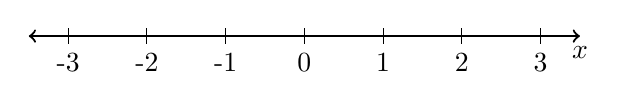
\begin{tikzpicture}
        \draw[thick, <->] (-3.5,0) -- (3.5,0) node[below] {$x$};

        \foreach \x in {-3,-2,-1,0,1,2,3}
            \draw (\x,0.1) -- (\x,-0.1) node[below] {\x};
    \end{tikzpicture}
\end{center}

We would represents the function as $\R$.

For two dimensions, we would would create two lines of real numbers and map them against each other.
\begin{center}
    \begin{tikzpicture}
        \draw[thick, <->] (-3.5,0) -- (3.5,0) node[below] {$x$};
    
        \draw[thick, <->] (0,-3.5) -- (0,3.5) node[left] {$y$};

        \foreach \x in {-3,-2,-1,1,2,3}
            \draw (\x,0.1) -- (\x,-0.1) node[below] {\x};
        
        \foreach \y in {-3,-2,-1,1,2,3}
            \draw (0.1,\y) -- (-0.1,\y) node[left] {\y};

    \end{tikzpicture}
\end{center}

For such a graph, we would represent the function as
\begin{align*}
    f : \R \rar \R
\end{align*}

Finally, for three dimensions we map a tuple of two to the real numbers.
\begin{center}
    \begin{tikzpicture}
        \draw[thick, <->] (-3.5,0,0) -- (3.5,0,0) node[below right] {$x$};
        \draw[thick, <->] (0,-3.5,0) -- (0,3.5,0) node[left] {$y$};
        \draw[thick, <->] (0,0,-3.5) -- (0,0,3.5) node[above] {$z$};

        \foreach \x in {-3,-2,-1,1,2,3}
            \draw (\x,0,0.1) -- (\x,0,-0.1) node[below] {\x};
        
        \foreach \y in {-3,-2,-1,1,2,3}
            \draw (0.1,\y,0) -- (-0.1,\y,0) node[left] {\y};

        \foreach \z in {-3,-2,-1,1,2,3}
            \draw (0,0.1,\z) -- (0,-0.1,\z) node[right] {\z};
    \end{tikzpicture}
\end{center}

Which we would represent with the function
\begin{align*}
    f : \R^2 \rar \R
\end{align*}

Or, for this course, it would be more helpful to think about these functions as,
\begin{align*}
    f(x,y) &= z
\end{align*}

We can formalize this definition as well.

\begin{definition}
    Suppose $f(x,y)$ is a \textbf{function of two variables}, then the set of all points $(x,y,z) \in \R^2$ such that $f(x,y) = z$ is the graph of
    $f(x,y)$ So, the points on teh graph are of the form $(x, y, f(x,y))$.
\end{definition}

Beyond the third dimension, graphical representations become difficult, but we can think about the relationships between input and outputs in terms of 
functions. For a function that maps $n$ variables to a real number, we would represent it as
\begin{align*}
    f : \R^n \rar \R.
\end{align*}

Or, more practically,
\begin{align*}
    f(x_1, ..., x_n) &= z.
\end{align*}

From now on, we'll focus primarily on three dimensions and generalizing formulas/tools to $n$ dimensions.

\subsection{Measuring Distance}
\begin{definition}
    Given two points $P_1(a_1, ..., a_n)$ and $P_2(b_1, ..., b_n)$, we can compute the \textbf{distance} with the following formula.
    \begin{align*}
        \sqrt{(b_1 - a_1)^2 + (b_2 - a_2)^2 + \cdots + (b_n - a_n)^2}
    \end{align*}
\end{definition}

\subsection{Generalizing Shapes}
We can start with shapes in lower dimensions and then express them in higher dimensions.

\begin{definition}
    \textbf{Translate} refers to the process of taking a function of fewer variables than dimensions and then extending it to more variables.
\end{definition}

\begin{definition}
    A \textbf{cylinder} refers to any function/shape that has been translated from its original dimensions to higher dimensions.
\end{definition}

For instance, if you were to take a point $x = 1$. You can translate it into $\R^2$ by representing it as the line $x = 1$.
Then, in three dimensions it would be a plane. In this case, the line and the plane are cylinders of the original point.

Similarly, you could start in the second dimension with a circle, then translate it into the third dimensions as a sphere. Here the sphere would
(somewhat counterintuitively) be the cylinder of the circle.

\subsection{Level Surfaces}
Sometimes it is difficult to graph a function by hand, so we rely on level surfaces.
\begin{definition}
    \textbf{Level surfaces} (sometimes known as \textbf{level curves}) are of the form
    \begin{align*}
        f(x,y) &= c \text{ for some constant $c \in \R$}
    \end{align*}

    \begin{example}
        Consider the function $f(x,y) = 100 - x^2 -y^2$.
        
        % \begin{center}
        %     \begin{tikzpicture}
        %         \begin{axis}[
        %             view={40}{40}, % Adjust the viewing angles
        %             colormap/viridis, % Color scheme
        %             axis lines=center,
        %             xlabel={$x$}, ylabel={$y$}, zlabel={$f(x,y)$},
        %             domain=-10:10,
        %             y domain=-10:10,
        %             samples=30, % Number of sample points
        %             samples y=30,
        %             enlargelimits=false,
        %             z buffer=sort
        %         ]
        %             \addplot3[surf] {100 - x^2 - y^2};
        %         \end{axis}
        %     \end{tikzpicture}
        % \end{center}

        For which the level curve would just be a bunch of circles. % upload graph maybe
    \end{example}

\end{definition}

\section{Vectors}

\subsection{Vector Basics}
Vectors are arrows pointing to different areas on a graph.

\begin{definition}
    Suppose $\vec{v}$ is a vector. If its initial point is at $(a_1,b_1)$ and its terminal point (with the arrow) is at $(a_2, b_2)$, then
    \begin{align*}
        \vec{v} &= \langle a_2 - a_1, b_2 - b_1 \rangle
    \end{align*}

    If $(a_1, b_1) = (0,0)$ (that is, it starts at the origin), then we call that vector a position vector.
\end{definition}

\subsubsection{Vector Properties}

\subsection{The Unit Vector}
\begin{definition}
    The \textbf{magnitude} or \textbf{length} of a vector, $\vec{v} = \langle a, b, c \rangle$ is found through the following formula.
    \begin{align*}
        | \vec{v} | &= \sqrt{a^2 - b^2 - c^2}
    \end{align*}

    The only vector with a length of zero is the zero vector. Vectors of length $1$ are called unit vectors.
\end{definition}

\begin{definition}
    A \textbf{unit vector} is a vector of length one. They are useful for when we want to describe the direction (but not magnitude) of a vector.
    Suppose theres a vector $\vec{v}$ which may or may not have a magnitude of $1$. We can find a vector that points in the same direction with the
    following formula.
    \begin{align*}
        \frac{\vec{v}}{|\vec{v}|}
    \end{align*}

    This basically just scales down the vector to a length of $1$.
\end{definition}

\begin{notation}
There are a few special unit vectors.
    \begin{align*}
        \hat{i} &= \langle 1, 0, 0 \rangle \\
        \hat{j} &= \langle 0, 1, 0 \rangle \\
        \hat{k} &= \langle 0, 0, 1 \rangle \\
    \end{align*}
\end{notation}

\subsection{The Dot Product (Inner Product)}
\begin{definition}
    Suppose $\vec{v} = \vect{a_1, a_2, a_3}$ and $\vec{u} = \vect{b_1, b_2, b_3}$. Then, the \textbf{dot product} or \textbf{inner product} is defined
    as the following.
    \begin{align*}
        \vec{v} \cdot \vec{u} &= a_1 b_1 + a_2 b_2 + a_3 b_3
    \end{align*}
\end{definition}

\begin{thm}
    If $\theta$ is the angle between two vectors $\vec{v}$ and $\vec{u}$, then 
    \begin{align*}
        \vec{v} \cdot \vec{u} &= |\vec{v}| |\vec{u}| \cos \gt
    \end{align*}

    Rearranging this equation, we get another helpful relationship.
    \begin{align*}
        \cos^{-1} \left( \frac{\vec{v} \cdot \vec{u}}{|\vec{v}| |\vec{u}|} \right) &= \gt
    \end{align*}
\end{thm}

\begin{corollary}
    If $\vec{v}$ and $\vec{u}$ are not zero vectors, then $\vec{v} \cdot \vec{u} = 0$ if and only if $\gt = 0$.
\end{corollary}

\subsubsection{Properties of the Dot Product}
\begin{align*}
    \vec{v} \cdot \vec{v} &= | \vec{v} |^2 \\
    \vec{v} \cdot \vec{u} &= \vec{u} \cdot \vec{v} \\
    \vec{v} \cdot (\vec{u} + \vec{w}) &= (\vec{v} \cdot \vec{u}) + (\vec{v} \cdot \vec{w}) \\
    (c \vec{v}) \cdot \vec{u} &= c(\vec{v} \cdot \vec{u}) = \vec{v} \cdot (c \vec{u}) 
\end{align*}

\subsection{The Cross Product}
\begin{definition}
    The \textbf{cross product} of two vectors $\vec{v} = \vect{a_1, a_2, a_3}$ and $\vec{u} = \vect{b_1, b_2, b_3}$ is defined as follows.
    \begin{align*}
        \vec{v} \times \vec{u} &= \vect{a_2 b_3 - a_3 b_2, - (a_1 b_3 - a_3 b_1), a_1 b_2 - a_2 b_1}
    \end{align*}
\end{definition}
\begin{thm}
    The cross product of $\vec{v}$ and $\vec{u}$ is orthogonal to both.
\end{thm}

\begin{thm}
    Let $\gt$ be the angle between $\vec{v}$ and $\vec{u}$. Then,
    \begin{align*}
        | \vec{v} \times \vec{u} | &= | \vec{v} | | \vec{u} | \sin \gt
    \end{align*}
\end{thm}

\begin{corollary}
    If $\vec{v}$ and $\vec{u}$ are not the zero vectors, then $\vec{v} \times \vec{u}$ if and only if $\vec{v}$ and $\vec{u}$ are orthonormal.
\end{corollary}

One last useful piece of information is that $\vec{v} \times \vec{u} = - \vec{u} \times \vec{v}$.

\subsubsection{Defining the Cross Product with the Determinant}

\begin{definition}
    The \textbf{determinant} in two dimensions is defined as follows.
    \begin{align*}
        \begin{vmatrix}
            a_1 & a_2 \\ 
            b_1 & b_2
        \end{vmatrix} &=
        a_1 b_2 - a_2 b_1
    \end{align*}

    Where you are functionally multiplying across the diagonals.

    In three dimensions, we define it as,
    \begin{align*}
        \left| \begin{array}{ccc}
            a_1 & a_2 & a_3 \\
            b_1 & b_2 & b_3 \\
            c_1 & c_2 & c_3
        \end{array} \right| &=
        a_1 \left| \begin{array}{cc}
            b_2 & b_3 \\ 
            c_2 & c_3
        \end{array} \right| -
        a_2 \left| \begin{array}{cc}
            b_1 & b_3 \\ 
            c_1 & c_3
        \end{array} \right| +
        a_3 \left| \begin{array}{cc}
            b_1 & b_2 \\ 
            c_1 & c_2
        \end{array} \right|
    \end{align*}
\end{definition}

\begin{lemma}
    Suppose you have two vectors, $\vec{v} = \vect{b_1, b_2, b_3}$ and $\vec{u} = \vect{c_1, c_2, c_3}$. The following property holds.
    \begin{align*}
        \vec{v} \times \vec{u} &= 
        \left| \begin{array}{ccc}
            \hat{i} & \hat{j} & \hat{k} \\
            b_1 & b_2 & b_3 \\
            c_1 & c_2 & c_3
        \end{array} \right|
    \end{align*}
\end{lemma}

\section{Planes}

\begin{definition}
    A \textbf{plane} in $\R^3$ is uniquely determined by a point in the plane $P_0 = (x_0, y_0, z_0)$ and the normal vector $\vec{n} = \vect{a, b, c}$.
    \begin{align*}
        ax + by + cz &= d
    \end{align*}

    For some constant $d$ such that $d = ax_0 + by_0 + cz_0$. So, the equation for a plane is more explicitly,
    \begin{align*}
        ax + by + cz &= ax_0 + by_0 + cz_0
    \end{align*}

    If you know a second point on the plane $P = (x, y ,z)$, you can derive this formula through the following method. First, find the vector
    between $P_0$ and $P$.
    \begin{align*}
        \vec{P_0 P} &= \vect{x - x_0, y - y_0, z - z_0}
    \end{align*}

    This produces a vector orthonormal to the plane (since its a point on the plane pointing to another point on the plane). Since the normal vector
    was defined to be normal to the plane, we know its also normal to this vector. So, the angle between the $\vec{n}$ and $\vec{P_0 P}$ is 
    $\frac{\pi}{2}$. Therefore,
    \begin{align*}
        \vec{n} \cdot \vec{P_0 P} &= 0 \\
        &= a(x - x_0) + b(y - y_0) + c(z - z_0)
    \end{align*}

    Isolating the constants to one side, this is exactly the equation of a plane.
\end{definition}

\begin{remark}
    Given three points on a plane, $P, Q, R$, you can find the normal vector (and the equation of the plane) by using the cross product.
    \begin{align*}
        \vec{n} &= \vec{P Q} \times \vec{PR}
    \end{align*}
\end{remark}

\section{Limits}

Limits operate in much of the same way as in single variable calculus. I won't dive into the specific definition since its a little convoluted and
unnecessary to know for our purposes. Know this: in single variable calculus, there are two ways to approach a limit, but in multivariable calculus,
there are an infinite number of ways to approach $(x,y) = (a,b)$. \textbf{For a limit to exist, all approaches must work. If even one of them doesn't
exist, then there is no limit. If you take to limits from different directions and they don't result in the same output, then the limit does not exist.}

There are a few types of functions that we know always have limits.
\begin{enumerate}
    \item Polynomial Functions
    \item ???
\end{enumerate}

So, if you can reduce a function into one of those forms (or rather manipulate it to show that it is one of those functions), then you know 
that function has a limit.

\begin{definition}
    The \textbf{partial derivative} of $f(x,y)$ with respect to $x$ is
    \begin{align*}
        \partd{f}{x} = \partd{z}{x} = f_x(x,y) = D_x f
    \end{align*}

    Where we take the derivative of $f$ as if $y$ was a constant.
\end{definition}



\include{sections/gradients}

\end{document}